\chapter[Circular Waveguide]{CIRCULAR WAVEGUIDE}
	Before we discuss the solution for the circular waveguide let us review what we discussed in the previous lecture and then discuss some important characteristics of the Bessel function when the order n is an integer.\\
	
	So as we have discussed, for a second order PDE of the form 
	 \begin{displaymath}
	 	x^2\frac{d^2y}{dx^2} + x\frac{dy}{dx} + (x^2-n^2)y {=} 0
	 \end{displaymath}
	 It is called a Bessel equation and one kind of the solution is called the Bessel function of the first kind given as an infinite series
	 \begin{displaymath}
	    J_n(x) {=} \sum^\infty_{k=0} \frac{(-1)^k (\frac{x}{2})}{k!\Gamma(n+k+1)}
	 \end{displaymath}
	 where n is the order of the solution and $\Gamma(n+k+1){=}(n+k)\Gamma(n+k)$. As we know for any second order PDE there is always two different independent solution and so we have another solution called the Bessel function of second kind or Neumann function given as 
	 \[Y_n(x) = \frac{\cos(n\pi)J_n(x)-J_{-n}(x)}{\sin(n\pi)} \]
	 In general the solution of the Bessel equation is \[y(x) = A J_n(x) + B Y_n(x)\]
	 However \[Y_n(0)=\pm\infty\] which means at the centre of a cylindrical symmetry the electromagnetic fields or power density are infinite at the centre which makes no physical sense. So due to practical reasons the solution of the Bessel function is 
	 \[y(x) = A J_n(x) \]
	 There is also the Bessel function of the third kind called the Henkel functions and they play important role in electro magnetics when dealing with dielectric waveguides such as the optical fibre where inside the waveguide we have the Bessel function of the first kind and outside the waveguide we have the Bessel functions of the third kind or Henkel functions.\\
	 
	 For all electromagnetic problem the order 'n' is always an integer. So we will have forms such as $ J_0(x) $, $ J_1(x) $, $ J_2(x) $, . and so on. Where only $J_0(x)$ has some value at x{=}0 while the rest value of n is zero is 
	 \[ J_n(0)=0 \; for \; n \neq 0 \]
	 If we plot these functions, we observe that the behaviour in similar to the sine and cosine function (which means it is periodic) but as x increases the peak value starts decreasing. For instance if we plot $J_0(x)$ as shown it peaks at x=0 and attenuates as x increases.
	 
	 \begin{figure}[H]
	 	\centering
	 	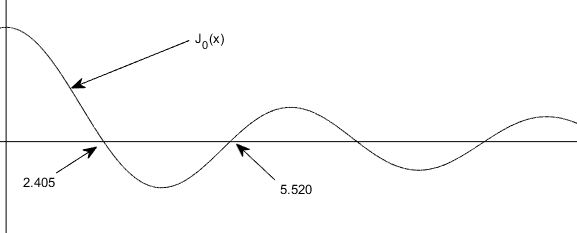
\includegraphics[height=5cm]{fig_1.1}
	 	\caption{}
	 	\label{fig:fig1}
	 \end{figure}
	 
	 
	 As we go to higher order functions the behaviour is similar to a sine function. Let's plot the $J_1(x)$ function as shown.
	 
	 \begin{figure}[H]
	 	\centering
	 	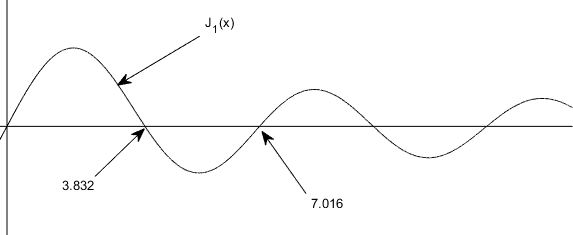
\includegraphics[height=5cm]{fig_2.1}
	 	\caption{}
	 	\label{fig:fig2}
	 \end{figure}
	 
	 So when looking for the solution for the waveguide there are two constraints involved and they are;
	 \begin{enumerate}
	 	\item What order n do we have for the solution.
	 	\item Which zero point (root) are we considering because the electric field has to get to zero point (root) at the boundary.
	 \end{enumerate}
	 So the first constraint, n tell us how the wave oscillate while the second constraint which we will denote with p, will tell us which zero point we are considering. 
	 \paragraph{} Therefore, a solution would be specified as $J_n^p(x)$ which gives a specific unique solution. For all possible solutions $J_n^p(x_{np})$, there would be a unique value of $x_{np}$, where $J_n^p(x_{np})=0$ given by the table below.
	 \begin{center}
	 	\begin{tabular}{|c|c c c|}
	 		\hline 
	 		\backslashbox{p}{n} & n=0 & n=1 & n=2 \\ 
	 		\hline 
	 		1&  2.405&  3.832& 5.136 \\ 
	 		
	 		2&  5.520&  7.016& 8.417 \\ 
	 		\hline 
	 	\end{tabular} 
	 \end{center}
	  The table above as we see tells us where the cut-off frequencies occurs for the circular waveguide. n and p in the circular waveguide is similar to m and n in the rectangular waveguide in a way such that they define the modes and the cut-off frequencies for each mode. We recall from the rectangular waveguide that m shows the number of peaks in the x direction while n shows the number of peaks in the y direction. However, in this case the two arguments n and p show what order of the solution and root of the solution we are considering.\\
	 
	 Now let's find the solution of the circular waveguide. Later on we will discuss the derivative of the Bessel function because it is needed in the solution of the waveguide when applying boundary condition.
	 
	 \section{TM mode in Circular Waveguide}
	 So we are considering a hollow metallic pipe of radius a, filled with a dielectric material of $\mu$ and $\epsilon$ as shown.
	 
	\begin{figure}[H]
		\centering
		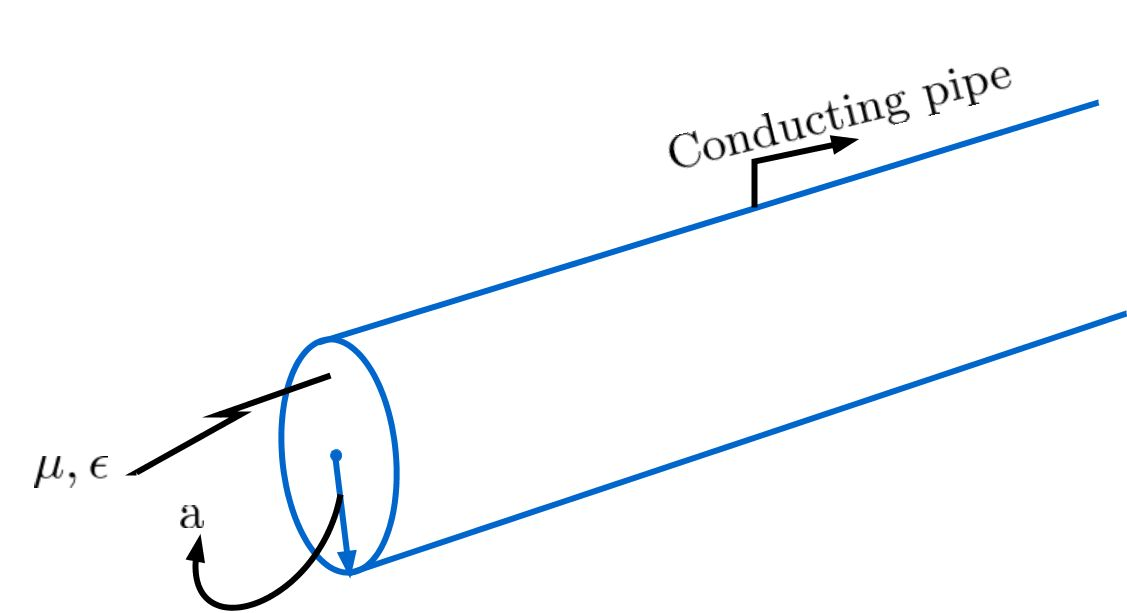
\includegraphics[width=0.7\linewidth]{fig_3.1}
		\caption{}
		\label{fig:fig3}
	\end{figure}
	 
	 For the Helmholtz wave equation 
	 \begin{equation}
	 	\bigtriangledown^2\vec{E} + w^2\mu\epsilon\vec{E}=0
	 	\label{eqn12.1}
	 \end{equation}\
	 The Laplacian term $\bigtriangledown^2\vec{E}$ has components in the transverse plane and longitudinal. We are still interested in the solution which is of the form of $\vec{E}=\vec{E}_{\bot}e^{-\gamma z}$ where the amplitude $\vec{E}_\bot$ remain in the transverse plane and the wave is propagating in the z direction with propagation constant $\gamma$. \\
	 So we will write equation \ref{eqn12.1} as:
	 \[\bigtriangledown^2\vec{E}_\perp e^{-\gamma z} + \omega^2 \mu\epsilon E_\perp e^{-\gamma z} = 0\]
	 where \[\bigtriangledown^2 = \bigtriangledown^2_\perp + \frac{\partial^2}{\partial z^2}\]
	 So 
	 \[\bigtriangledown^2_\perp\vec{E}_\perp e^{-\gamma z} + \frac{\partial^2}{\partial z^2}\left(\vec{E}_\perp e^{-\gamma z}\right) + \omega^2\mu\epsilon\vec{E}_\perp e^{-\gamma z} = 0\]
	 \[\bigtriangledown^2_\perp\vec{E}_\perp e^{-\gamma z} + (\gamma^2)\left(\vec{E}_\perp e^{-\gamma z}\right) + \omega^2\mu\epsilon\vec{E}_\perp e^{-\gamma z} = 0\]
	 \[\bigtriangledown^2_\perp\vec{E}_\perp e^{-\gamma z} + (\omega^2\mu\epsilon + \gamma^2)\left(\vec{E}_\perp e^{-\gamma z}\right) = 0\]
	 \begin{equation}
	 	\bigtriangledown^2_\perp\vec{E}_\perp + (\omega^2\mu\epsilon + \gamma^2)\vec{E}_\perp = 0
	 	\label{eqn12.2}
	 \end{equation}
	 where $h^2 = \omega^2\mu\epsilon + \gamma^2$. To solve this equation we will use the cylindrical coordinate system. We recall for the rectangular waveguide, we used the Cartesian coordinate system because irrespective of the location we consider along x in the transverse plane the limits along y direction is the same. However for a circular waveguide whose transverse plane is a circle, the limits of y at any location along x changes and so it is preferable to solve the equation using the cylindrical coordinate system because the wave guide has a cylindrical symmetry.\\
	 
	 The cylindrical coordinate system is defined by $\hat{r}$ and $\hat{\phi}$ in the transverse plane and $\hat{z}$ in the longitudinal direction.
	   
	 \begin{figure}[H]
	   	\centering
	   	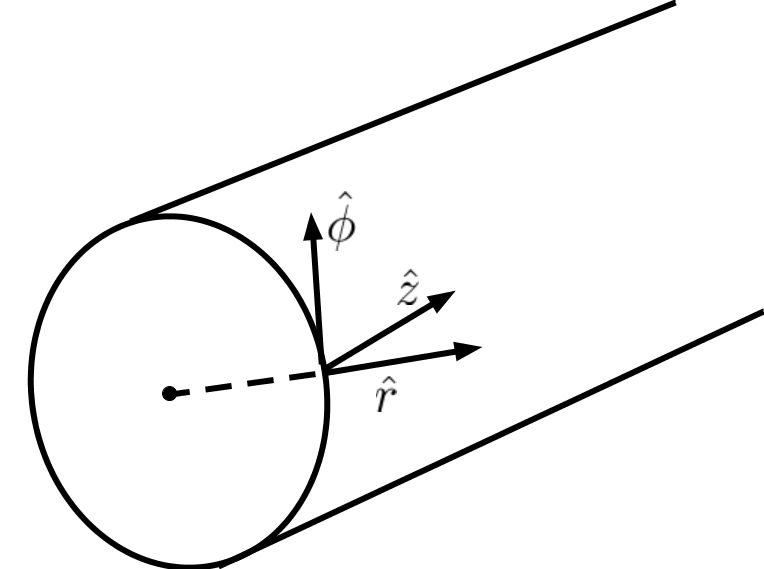
\includegraphics[height=5cm]{fig_4.1}
	   	\caption{}
	   	\label{fig:fig4}
	 \end{figure}
	   
	   
	 We will now write equation \ref{eqn12.2} for the cylindrical coordinate as 
	   
	 $$
	 \frac{1}{r}\frac{\partial}{\partial r}(r\frac{\partial^2\vec{E}_\bot}{\partial r}) + \frac{1}{r^2}\frac{\partial^2\vec{E}_\bot}{\partial\phi^2}+ h^2\vec{E}_\bot = 0 
	 $$
	 which is the equation which will give the solution of the modes. 
	 \\ The field components in the circular waveguide are $E_r$, $E_\phi$ and $E_z$ as shown
  
     \begin{figure}[H]
       	\centering
      	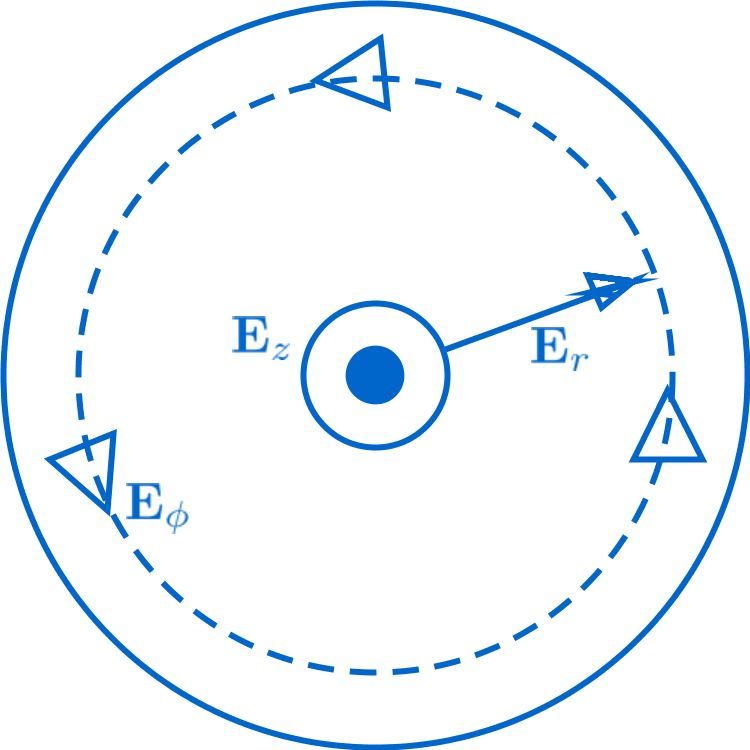
\includegraphics[height=5cm]{fig_5.1}
       	\caption{}
       	\label{fig:fig5}
     \end{figure}
   
	  For the TM mode we know that $H_z=0$ and $E_z$ exists and for the TE mode $E_z=0$ and $H_z$ will exist. Therefore, for the TM mode we should solve for $E_z$ with appropriate boundary conditions and for TE mode, we should solve for $H_z$ with appropriate boundary conditions. \\
	  
	  So for the TM mode we will solve for $E_z$ which should vary in r and $\phi$ and propagates in the z direction as shown $E_z(r,\phi, z)=E_z(r,\phi)e^{-\gamma z}$, where $e^{-\gamma z}$ signifies the field is propagating in the z direction. So from the wave equation for the cylindrical coordinate which we have written, we have;
	  \begin{equation}
	  	\frac{1}{r}\frac{\partial}{\partial r}(r\frac{\partial E_z}{\partial r}) + \frac{1}{r^2}\frac{\partial^2 E_z}{\partial\phi^2} + h^2 E_z = 0 
	  	\label{eqn12.3}
	  \end{equation}
	 
	  And we know r and $\phi$ are orthogonal so whatever variation we have in r is not related to the variations in $\phi$ so we can write $E_z(r, \phi)$ as
	  $$
	  E_z(r, \phi) = R(r)\Phi(\phi) 
	  $$
	  using separation of variables where $R(r)$ is a function of r only and $\Phi(\phi)$ is a function of $\phi$ only.
	  \\
	  So we will write equation \ref{eqn12.3} as 
	  $$ 
	  \frac{1}{r}\frac{\partial}{\partial r}(r\frac{\partial(R(r)\Phi(\phi))}{\partial r}) + \frac{1}{r^2}\frac{\partial^2 (R(r)\Phi(\phi)}{\partial \phi^2}) + h^2E_z(r,\phi) = 0
	  $$
	  $$
	  \frac{\Phi(\phi)}{r}\frac{d}{dr}\left(r\frac{dR(r)}{dr}\right) + \frac{R}{r^2}\frac{d^2\Phi(\phi)}{d\phi^2} + h^2 E_z = 0
	  $$
	  Divide through by $E_z(r, \phi)=R(r)\Phi(\phi)$ gives 
	  $$
	  \frac{1}{rR(r)}\frac{d}{dr}\left(r\frac{dR(r)}{dr}\right) + \frac{1}{r^2\Phi(\phi)}\frac{d^2\Phi(\phi)}{d\phi^2} + h^2 = 0
	  $$
	  multiply through by $r^2$
	  $$
	  \frac{r}{R(r)}\frac{d}{dr}\left(r\frac{dR(r)}{dr}\right) + \frac{1}{\Phi(\phi)}\frac{d^2\Phi(\phi)}{d\phi^2} + r^2h^2=0
	  $$
	 \begin{equation}
	     \underbrace{\frac{r}{R(r)}\frac{d}{dr}\left(r\frac{dR(r)}{dr}\right)	+ r^2 h}_{function \; of\; r \; only} 
	   	   + \underbrace{\frac{1}{\Phi(\phi)}\frac{d^2\Phi(\phi)}{d\phi^2}}_{function \; of \; \phi \; only} = 0 
	   	   \label{eqn12.4} 
	 \end{equation}
	    
	  which is true for any value of r and $\phi$. The above equation can only be true if each function is a constant and lets denote the constant as $-n^2$ for the function of $\phi$ only ie. 
	  \begin{equation}
	    \frac{1}{\Phi(\phi)}\frac{d^2\Phi(\phi)}{d\phi^2}=-n^2 \; \; => \;\; \frac{d^2\Phi(\phi)}{d\phi^2} + n^2\Phi(\phi) = 0
	    \label{eqn12.5}
	  \end{equation}
	  And so $\frac{r}{R(r)}\frac{d}{dr}(r\frac{dR(r)}{dr}) + r^2h$ has to be $+n^2$ so that equation \ref{eqn12.4} holds, hence;
	  $$
	  \underbrace{\frac{r}{R(r)}\frac{d}{dr}\left(r\frac{dR(r)}{dr}\right)} + r^2h-n^2=0
	  $$
	  $$
	  \frac{r^2}{R(r)}\frac{d^2R(r)}{dr^2} + \frac{r}{R(r)}\frac{dR(r)}{dr} - r^2h-n^2=0
	  $$
	  Multiply through by $\frac{R(r)}{r^2}$
	  \begin{equation}
	   	\frac{d^2R(r)}{dr^2}+\frac{1}{r}\frac{dR(r)}{dr} + (h^2-\frac{n^2}{r^2})R(r)=0
	   	\label{eqn12.6}
	  \end{equation}
	   
	  which in a Bessel equation and can be compared to 
	  $$
	  \frac{d^2y}{dx^2}+\frac{1}{x}\frac{dy}{dx}+\left(1-\frac{n^2}{x^2}\right)y = 0
	  $$
	  and recall $n^2$ is the constant we introduced. First lets solve the second order ordinary differential equation given in equation \ref{eqn12.5} as
	  $$
	  \frac{d^2\Phi(\phi)}{d\phi^2} + n^2\Phi(\phi) = 0
	  $$
	  whose solution is $\Phi(\phi)\equiv $ either $\sin(n\phi)$ or $\cos(n\phi)$. Whether we choose $\sin(n\phi)$ or $\cos(n\phi)$ is immaterial. It only changes the location of reference $\phi=0$ angle in the $\phi$ direction.\\ 
	  
	  By convention we choose $\cos(n\phi)$ so that one solution becomes
	  $$
	  \Phi(\phi)=A\cos(n\phi)
	  $$
	  which will be periodic about $2\pi$ if n is an integer so n has to be an integer.\\
	  
	  Also the solution of the Bessel equation, equation \ref{eqn12.6} is a Bessel function and it is given as
	  $$
	  R(r)=CJ_n(hr)
	  $$
	  The argument of the Bessel function is hr if we compare the two equation below
	  $$
	  r^2\frac{d^2R(r)}{dr^2} + r\frac{dR(r)}{dr} + ((hr)^2 - n^2)R(r) = 0
	  $$
	  $$
	  x^2\frac{d^2y}{dx^2} + x\frac{dy}{dx} + (x^2-n^2)y=0
	  $$
	  Therefore $E_z(r,\phi) = C_nJ_n(hr)\cos(n\phi)$ where $C_n$ depends on the mode we are considering.\\
	  
	  The other components can be gotten from the expressions below for the transverse field component we have discussed in previous lectures.
	  $$
	  \vec{E}_\bot=\frac{-j\omega\mu}{h^2}\bigtriangledown_\bot\times H_z\hat{z} - \frac{\gamma}{d^2}\bigtriangledown_\bot E_z
	  $$
	  and
	  $$
	  \vec{H}_\bot = \frac{-j\omega\mu}{h^2}\bigtriangledown_\bot\times E_z\hat{z}-\frac{\gamma}{h^2}\bigtriangledown_\bot H_z
	  $$
	  We recall for the TM mode $H_z=0$
	  so
	  $$
	  \vec{E}_\bot=-\frac{\gamma}{h^2}\bigtriangledown_\bot E_z$$ for a lossless medium $$\gamma=j\beta
	  $$
	  therefore 
	  $$
	  \vec{E}_\bot = \frac{-j\beta}{h^2}\bigtriangledown_\bot E_z
	  $$
	  $$
	  \vec{E}_\bot = \frac{-j\beta}{h^2}\left\{\frac{\hat{r}\partial E_z}{\partial r} + \frac{\hat{\phi}}{r}\frac{\partial E_z}{\partial\phi} \right\}
	  $$
	  so that 
	  $$
	  E_r=\frac{-j\beta}{h^2}\frac{\partial}{\partial r}E_z = \frac{-j\beta}{h^2}C_nJ'_n(hr)\cos(n\phi)
	  $$
	  $$
	  E_\phi = \frac{-j\beta\partial}{h^2r\partial}E_z = \frac{j\beta n}{h^2 r}C_nJ_n(hr)\sin(n\phi)
	  $$
	  Also for transverse components $H_r$ and $H_\phi$ \\ we have
	  $$
	  \vec{H}_\bot=\frac{j\omega\epsilon}{h^2}\bigtriangledown_\bot\times(E_z\hat{z})
	  $$
	  $$
	  =\frac{j\omega\epsilon}{h^2}\left\{
	  \frac{1}{r}
	  	\begin{tabular}{| c c c |}
	     	$\hat{r}$ &$r\hat{\phi}$ &$\hat{z}$ \\ $\frac{\partial}{\partial r}$ &$\frac{\partial}{\partial\phi}$&0 
	     	\\ 0 & 0 &$\hat{E}_z$
	     \end{tabular}
	     \right\}
	  $$
	  $$
	  H_r=\frac{j\omega\epsilon }{h^2r}\frac{\partial E_z}{\partial \phi} = \frac{-j\omega\epsilon n}{h^2r}C_nJ_n(hr)\sin(n\phi)
	  $$
	  and \[H_\phi = -\frac{j\omega\epsilon}{h^2}\frac{\partial}{\partial r}E_z = -\frac{j\omega\epsilon}{h^2}C_nJ'_n(hr)\cos(n\phi)\]
	  where $J_n'(hr)$ is the derivative of the Bessel function. Now let's determine h by applying the boundary conditions.\\
	  
	  The $E_z$ component is given as $C_nJ_n(hr)\cos(n\phi)$ is parallel or tangential to the conducting wall and so $E_z(r=a)=0$. This implies that $J_n(ha)=0$ which could be any root of a specific Bessel function as n {=} 0,1,2,.... Let's consider n = 0 which is the first order Bessel function $J_0(hr)$. Also n=0 implies that there is a constant field in the $\phi$ direction since $\cos(n\phi)=1$. In general, n shows the number of wavelength, $\lambda$ that fits within $2\pi$ and the order of the Bessel function. For n=0 if we consider the first root of the Bessel function $J_0(hr)$ to satisfy the boundary condition at r=a we have that $h_a = 2.405$ from the table below
	     \begin{center}
	     	\begin{tabular}{| c | c c c |}
	     		\hline
	     		\backslashbox{p}{n} &n{=}0 &n{=}1 &n{=}2 \\
	     		\hline
	     		1 &2.405 &3.832 &5.136 \\
	     		2 &5.520 &7.016 &8.417 \\
	     		\hline
	     	\end{tabular}
	     \end{center}
	     
 
      Also $J_0(ha)=0$ if $ha=5.520$ for the second root at p=2. The first case is called $TM_{01}$ mode and the second case is called the $TM_{02}$ mode.
      
      \begin{figure}[H]
      	\centering
      	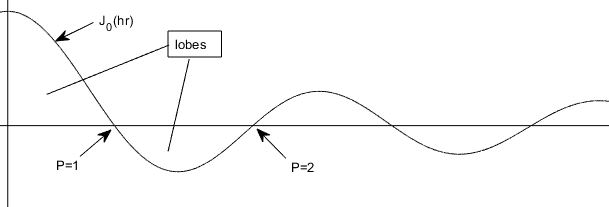
\includegraphics[height=5cm]{fig_6.1}
      	\caption{}
      	\label{fig:fig6}
      \end{figure}
      
      Therefore $J_n^p(hr)$ corresponds to $TM_{np}$ mode where n tells us the number of wavelengths $\lambda$ that is in the $\phi$ direction and p tells us the number of lobes that is in the r direction.
      \\ The fundamental TM mode in the $TM_{01}$ mode which has 
      $$
         ha = 2.405 \ \ => \ \ h=\frac{2.405}{a}
      $$
      from $h^2=\gamma^2+w^2\mu\epsilon $ at cut-off, the propagation constant for a lossless medium is zero since $\gamma=j\beta$ and $\beta=0$ as there is no propagation through the conducting wall. 
      \\ So
      $$
        h^2=\omega_c^2\mu\epsilon
      $$ where $\omega_c$ is the cut-off frequency in radians given as $2\pi f_c$ and $f_c$ is the cut-off frequency in Hertz.
      \\So $f_c =\frac{h}{2\pi\sqrt{\mu\epsilon}}$, for $TM_{01}$ mode $h=\frac{2.405}{a}$ therefore 
      $$
      f_c=\frac{2.405}{2\pi a\sqrt{\mu\epsilon}} =\frac{0.383}{a\sqrt{\mu\epsilon}}
      $$
      The second TM mode is the $TM_{11}$ mode where $ha =3.832$ such that $h=\frac{3.832}{a}$ and $f_c=\frac{3.832}{2\pi a\sqrt{\mu\epsilon}}$. Also, the next mode is the $TM_{21}$ mode for which $ha =5.136$ and $h=\frac{5.136}{a} \Longrightarrow f_c=\frac{5.136}{2\pi a \sqrt{\mu\epsilon}}$ and so on. \\
      Let's examine the fundamental mode $TM_{01}$ briefly. Here n=0 which implies that only the fields $E_r, \; E_z \; and \; H_\phi$ exists and they are not varying in the $\phi$ direction. They are given as
      $$
        E_r=\frac{-j\beta}{h^2}C_0J_0'(hr)
      $$
      $$
        E_z=C_oJ_o(hr)
      $$
      and
      $$
        H_\phi=\frac{j\omega\epsilon}{h^2}C_0J_0'(hr)
      $$
      
      From our study of Bessel function of the first order, $J_0(hr)$ is maximum at hr=0 which is the centre of the waveguide so we expect $E_z$ to vary in the r direction such that it is maximum at the centre ant it reduces to zero for the first root at the surface. The two dimensional plots will be treated in the next lecture for different TM modes where we can visually see the changes in the magnitudes of fields in the waveguide.